\section{State of the Art}

\subsection{Classical \gls{eeg}-based Models}

Early developments of \gls{bci} systems based on \gls{eeg} and \gls{mi} paradigms have been fundamentally constrained by the physical and physiological properties of \gls{eeg} signal acquisition. Due to volume conduction effects, neural electrical activity generated at cortical sources propagates through heterogeneous tissue layers before being recorded at the scalp, leading to spatial blurring and mixing of neural sources across electrodes \cite{wang2019eeg}. This phenomenon severely limits the spatial resolution of \gls{eeg} recordings, reducing the ability to localize task-related cortical activations and impairing the discriminative power of sensor-level representations. Consequently, early \gls{bci} systems relied heavily on signal processing techniques designed to enhance task-relevant information while attempting to suppress noise and spatial interference \cite{singh2021comprehensive}.

Classical \gls{eeg} decoding pipelines typically employ spectral and time--frequency transformations to extract features associated with \gls{mi} activity. Methods based on Fourier analysis and wavelet decompositions have been widely used to isolate oscillatory patterns within the $\mu$ and $\beta$ bands, which are known to reflect sensorimotor rhythms modulated during \gls{mi} tasks \cite{pfurtscheller1999event,singh2021comprehensive}. While these representations partially address the nonstationary nature of \gls{eeg} signals by enabling localized spectral analysis, they do not inherently resolve the spatial ambiguity introduced by volume conduction, as frequency-domain features remain derived from mixed sensor-level signals.

To enhance spatial discriminability, classical approaches frequently incorporate spatial filtering techniques, most notably \gls{csp} and its extensions, such as \gls{fbcsp}. By projecting multichannel \gls{eeg} signals into a discriminative subspace that maximizes variance differences between classes, \gls{csp}-based methods can improve signal-to-noise ratio and classification accuracy under controlled experimental conditions \cite{wang2019eeg}. However, these methods rely on linear assumptions and are highly sensitive to noise, electrode placement, and inter-subject variability. Furthermore, their dependence on predefined frequency bands and subject-specific calibration procedures significantly limits their robustness and generalization capability, particularly in subject-independent or clinical scenarios \cite{maswanganyi2022statistical,saha2020intra}.

Additional preprocessing strategies, including surface Laplacian filtering, have been proposed to mitigate the effects of volume conduction by emphasizing local cortical activity and suppressing global signal components. Although such techniques can improve spatial resolution at the sensor level, they remain vulnerable to residual noise and cannot fully disentangle underlying cortical sources, resulting in only partial mitigation of spatial mixing \cite{wang2019eeg,pan2025enhancing}. As a result, classical \gls{eeg}-based \gls{bci} systems often exhibit limited robustness and reduced interpretability, especially when deployed in real-world environments characterized by high noise levels and pronounced inter-subject variability \cite{bouazizi2024interpretability}.{These main limitations of classical \gls{eeg}-based decoding pipelines are summarized in Figure~\ref{fig:classical_eeg_models}.}

% \begin{figure}[H]
% \centering
% \begin{tikzpicture}[x=\linewidth,y=1.2cm,line width=0.9pt,font=\normalsize]

% % ===== spacing =====
% \def\labelpad{0.015}
% \def\topbot{0.10}
% \def\dy{0.9}
% \def\yA{1.0}
% \def\gapBlocks{0.9} % <<< gap vertical (en "unidades y") entre grupos
% \def\amp{3pt}

% \pgfmathsetmacro{\yB}{\yA - (2 + \gapBlocks)*\dy}

% % ===== styles =====
% \tikzset{
%   brace/.style={
%     draw=none,
%     postaction={draw,decorate,decoration={brace,mirror,raise=0pt,amplitude=\amp}}
%   },
%   lab/.style={anchor=east,fill=white,inner sep=1.2pt,align=center},
%   glab/.style={anchor=east,fill=white,inner sep=1.2pt},
%   item/.style={anchor=west,text width=0.50\linewidth}
% }

% % ===== column positions =====
% \pgfmathsetmacro{\xMain}{0.30}
% \pgfmathsetmacro{\xInner}{0.53}
% \pgfmathsetmacro{\xText}{0.55}

% % ===== labels =====
% \def\Main{Classical EEG-based \\ Models}
% \def\A{Spectral / Spatial}
% \def\B{Classification}

% % ===== items =====
% \def\Aone{Fourier / Wavelet features $\rightarrow$
% \textcolor{red}{limited spatial specificity}}

% \def\Atwo{STFT / Time--frequency $\rightarrow$
% \textcolor{red}{sensor-level source mixing}}

% \def\Athree{CSP / FBCSP $\rightarrow$
% \textcolor{red}{linear assumptions, noise sensitivity}}

% \def\Afour{Surface Laplacian $\rightarrow$
% \textcolor{red}{partial mitigation of volume conduction}}

% \def\Bone{LDA $\rightarrow$
% \textcolor{red}{subject-dependent calibration}}

% \def\Btwo{SVM $\rightarrow$
% \textcolor{red}{poor generalization across subjects}}

% % ===== main brace =====
% \draw[brace] (\xMain,\yA+1.5*\dy+\topbot) -- (\xMain,\yB-0.5*\dy-\topbot);
% \node[lab] at (\xMain-\labelpad, {(\yA+\yB)/2}) {\Main};

% % ===== group braces (SEGUND A ETAPA: separados de verdad) =====

% % Spectral/Spatial brace (4 items: yA±1.5dy)
% \draw[brace]
%   (\xInner,\yA+1.5*\dy+\topbot) --
%   (\xInner,\yA-1.5*\dy-\topbot);

% % Classification brace (2 items: yB±0.5dy)
% \draw[brace]
%   (\xInner,\yB+0.5*\dy+\topbot) --
%   (\xInner,\yB-0.5*\dy-\topbot);

% % ===== group labels =====
% \node[glab] at (\xInner-0.01,\yA) {\A};
% \node[glab] at (\xInner-0.05,\yB) {\B};

% % ===== items =====
% \node[item] at (\xText,\yA+1.5*\dy) {\Aone};
% \node[item] at (\xText,\yA+0.5*\dy) {\Atwo};
% \node[item] at (\xText,\yA-0.5*\dy) {\Athree};
% \node[item] at (\xText,\yA-1.5*\dy) {\Afour};

% \node[item] at (\xText,\yB+0.5*\dy) {\Bone};
% \node[item] at (\xText,\yB-0.5*\dy) {\Btwo};

% \end{tikzpicture}
% \vspace{-2em}
% \caption{Fundamental limitations of classical \gls{eeg}-based models for \gls{mi} decoding. Classical pipelines rely on handcrafted spectral and spatial features combined with shallow classifiers, which remain constrained by low spatial resolution, linear assumptions, sensitivity to noise, and strong subject dependence.}
% \label{fig:classical_eeg_models}
% \end{figure}

%-----------------------------------------------
\begin{figure}[htbp]
\centering

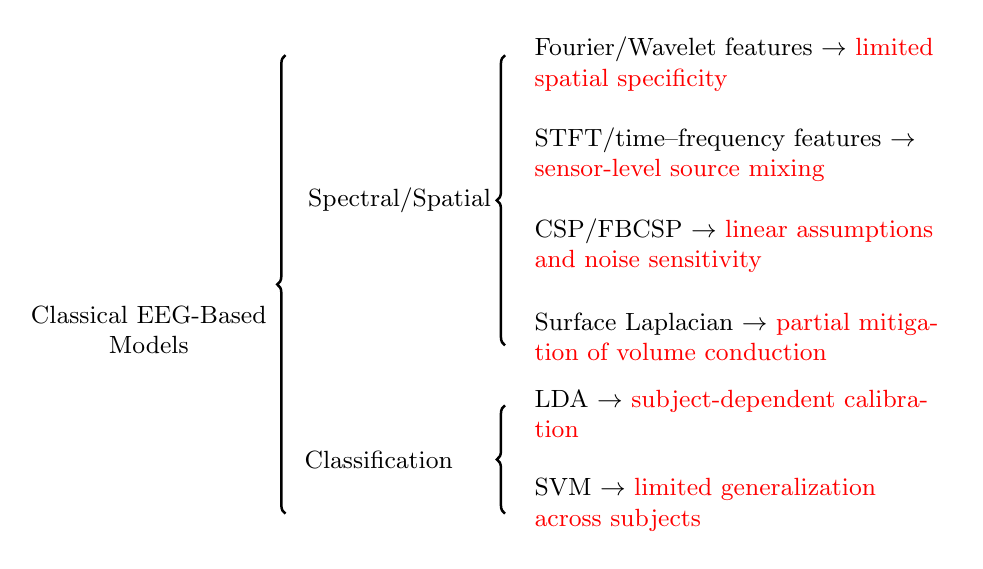
\begin{tikzpicture}[
    x=\linewidth,
    y=1.1cm,
    line width=0.9pt,
    font=\small
]

% ===== Spacing =====
\def\labelpad{0.015}
\def\topbot{0.10}
\def\dy{1.05}
\def\yA{1.0}
\def\gapBlocks{0.85}
\def\amp{3pt}

\pgfmathsetmacro{\yB}{\yA-(2+\gapBlocks)*\dy}

% ===== Styles =====
\tikzset{
    brace/.style={
        draw=none,
        postaction={
            draw,
            decorate,
            decoration={
                brace,
                mirror,
                raise=0pt,
                amplitude=\amp
            }
        }
    },
    lab/.style={
        anchor=east,
        fill=white,
        inner sep=1.2pt,
        align=center
    },
    glab/.style={
        anchor=east,
        fill=white,
        inner sep=1.2pt,
        align=center
    },
    item/.style={
        anchor=west,
        text width=0.43\linewidth,
        align=left
    }
}

% ===== Column positions =====
\pgfmathsetmacro{\xMain}{0.30}
\pgfmathsetmacro{\xInner}{0.53}
\pgfmathsetmacro{\xText}{0.55}

% ===== Labels =====
\def\Main{Classical EEG-Based\\Models}
\def\A{Spectral/Spatial}
\def\B{Classification}

% ===== Items =====
\def\Aone{Fourier/Wavelet features $\rightarrow$
\textcolor{red}{limited spatial specificity}}

\def\Atwo{STFT/time--frequency features $\rightarrow$
\textcolor{red}{sensor-level source mixing}}

\def\Athree{CSP/FBCSP $\rightarrow$
\textcolor{red}{linear assumptions and noise sensitivity}}

\def\Afour{Surface Laplacian $\rightarrow$
\textcolor{red}{partial mitigation of volume conduction}}

\def\Bone{LDA $\rightarrow$
\textcolor{red}{subject-dependent calibration}}

\def\Btwo{SVM $\rightarrow$
\textcolor{red}{limited generalization across subjects}}

% ===== Main brace =====
\draw[brace]
    (\xMain,\yA+1.5*\dy+\topbot) --
    (\xMain,\yB-0.5*\dy-\topbot);

\node[lab]
    at (\xMain-\labelpad,{(\yA+\yB)/2})
    {\Main};

% ===== Group braces =====

% Spectral/Spatial group
\draw[brace]
    (\xInner,\yA+1.5*\dy+\topbot) --
    (\xInner,\yA-1.5*\dy-\topbot);

% Classification group
\draw[brace]
    (\xInner,\yB+0.5*\dy+\topbot) --
    (\xInner,\yB-0.5*\dy-\topbot);

% ===== Group labels =====
\node[glab] at (\xInner-0.01,\yA) {\A};
\node[glab] at (\xInner-0.05,\yB) {\B};

% ===== Spectral/Spatial items =====
\node[item] at (\xText,\yA+1.5*\dy) {\Aone};
\node[item] at (\xText,\yA+0.5*\dy) {\Atwo};
\node[item] at (\xText,\yA-0.5*\dy) {\Athree};
\node[item] at (\xText,\yA-1.5*\dy) {\Afour};

% ===== Classification items =====
\node[item] at (\xText,\yB+0.5*\dy) {\Bone};
\node[item] at (\xText,\yB-0.5*\dy) {\Btwo};

\end{tikzpicture}

\vspace{0.8em}

\caption{Fundamental limitations of classical
\gls{eeg}-based models for \gls{mi} decoding. Classical pipelines
rely on handcrafted spectral and spatial features combined with
shallow classifiers, which remain constrained by low spatial
resolution, linear assumptions, sensitivity to noise, and strong
subject dependence.}
\label{fig:classical_eeg_models}

\end{figure}
%-----------------------------------------------

\subsection{Connectivity-based Methods for  \gls{eeg}-based \gls{bci}}

Beyond classical spectral and spatial pipelines, connectivity-based methods have emerged as a key strategy for modeling inter-channel interactions in \gls{eeg}-based \gls{bci} systems, particularly to address the nonlinear and nonstationary nature of neural dynamics \cite{shoka2019literature,singh2021comprehensive}. {The main challenges that motivate this connectivity-based perspective, including temporal drift, linear-connectivity limitations, volume conduction effects, and the need for directed nonlinear measures, are summarized in Figure~\ref{fig:nonlinear_nonstationary_dependencies}.} {\gls{eeg} signals reflect the collective activity of large-scale neural populations whose interactions evolve over time as a function of attention, fatigue, and task engagement~\cite{wang2019eeg}.} In paradigms such as \gls{mi} and in \gls{eeg}-based applications targeting neurological and neurodevelopmental conditions, including \gls{adhd}, these temporal variations induce pronounced changes in the statistical properties of \gls{eeg} signals both within and across trials, violating the stationarity assumptions underlying many classical signal processing and machine learning approaches. As a result, representations derived from fixed temporal or spectral assumptions often fail to capture the dynamic structure of brain activity, limiting robustness and reliability \cite{singh2021comprehensive}.

Early attempts to model inter-channel relationships in \gls{eeg} primarily relied on linear and symmetric measures of functional connectivity, such as correlation, coherence, and phase-based metrics \cite{pereda2005nonlinear}. While these measures provide valuable insights into synchronized neural activity, they are inherently limited in their expressive power, as they assume linear interactions and fail to distinguish between driving and responding neural sources \cite{bastos2016tutorial}. Moreover, linear connectivity measures are particularly vulnerable to volume conduction effects, often producing spurious connections that reflect common-source artifacts rather than genuine neural interactions \cite{nunez1997eeg,vinck2011improved}. These limitations become especially critical in scenarios characterized by high inter- and intra-subject variability, such as \gls{mi}-based decoding and \gls{eeg}-based studies involving \gls{adhd}, where fluctuations in attention and cognitive state further complicate the reliable characterization of brain network dynamics.

To overcome these limitations, increasing attention has been devoted to information theoretic and causality-based measures capable of capturing nonlinear  and directed interactions between \gls{eeg} channels. Among these, \gls{te} has emerged as a principled framework for quantifying directed information flow between time series, enabling the identification of asymmetric and time-delayed dependencies that cannot be detected by correlation-based methods \cite{staniek2008symbolic}. By explicitly modeling how the past of one signal reduces uncertainty about the future of another, \gls{te} provides a more faithful representation of effective brain connectivity, closely aligning with the notion of neural communication and causal influence \cite{bastos2016tutorial,faes2017information}.

Despite its theoretical appeal, the practical application of \gls{te} to \gls{eeg} data remains challenging. Classical estimators require explicit probability density estimation, which is highly sensitive to noise, data length, and dimensionality \cite{vicente2011transfer}. These challenges are exacerbated in \gls{eeg} recordings, where limited trial counts, nonstationarity, and high-dimensional inter-channel interactions hinder reliable connectivity estimation \cite{zhang2015bayesian,faes2017information}. As a result, many studies restrict \gls{te} analysis to small subsets of channels or rely on simplified assumptions that compromise the fidelity of the inferred connectivity patterns.

More recently, research has explored kernel-based and embedding-based formulations to alleviate some of these challenges, enabling more robust estimation of nonlinear dependencies without explicit density modeling \cite{marinazzo2011kernel}. In parallel, deep learning approaches have begun to incorporate connectivity information as part of the feature representation, either by using precomputed connectivity matrices or by embedding interaction patterns directly into neural architectures \cite{li2019deep,rolls2022effective}. While these methods improve interpretability and provide richer representations of brain dynamics, they often rely on externally computed and fixed connectivity estimators, preventing joint optimization with the classification objective and limiting adaptability to task-specific dynamics.

\begin{figure}[H]
\centering
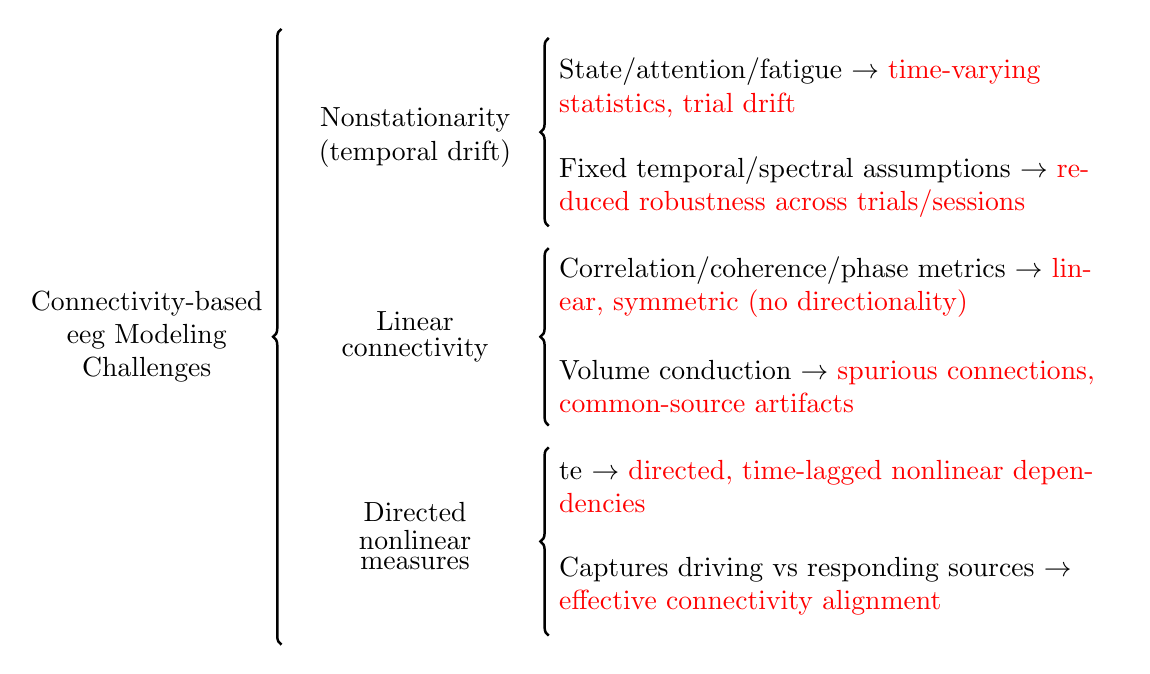
\begin{tikzpicture}[x=\linewidth,y=1.15cm,line width=0.9pt,font=\normalsize]

% ===== spacing =====
\def\labelpad{0.015}
\def\topbotMain{0.10}
\def\topbotInner{0.00}
\def\dy{1.1}
\def\yT{2.35}
\def\amp{3pt}
\def\vgap{0.12}

% ===== styles =====
\tikzset{
  brace/.style={
    draw=none,
    postaction={draw,decorate,decoration={brace,mirror,raise=0pt,amplitude=\amp}}
  },
  lab/.style={anchor=east,fill=white,inner sep=1.2pt,align=center},
  glab/.style={anchor=center,fill=white,inner sep=1.2pt,align=center},
  item/.style={anchor=west,text width=0.58\linewidth}
}

% ===== column positions =====
\pgfmathsetmacro{\xMain}{0.28}
\pgfmathsetmacro{\xInner}{0.56}
\pgfmathsetmacro{\xText}{0.56}
\pgfmathsetmacro{\xMid}{(\xMain+\xInner)/2}

% ===== labels =====
\def\Main{\shortstack{Connectivity-based\\\gls{eeg} Modeling\\Challenges}}

\def\GOne{\shortstack{Nonstationarity\\(temporal drift)}}
\def\GTwo{\shortstack{Linear\\connectivity}}
\def\GThree{\shortstack{Directed\\nonlinear\\measures}}

% ===== items =====
\def\Ione{State/attention/fatigue $\rightarrow$ \textcolor{red}{time-varying statistics, trial drift}}
\def\Itwo{Fixed temporal/spectral assumptions $\rightarrow$ \textcolor{red}{reduced robustness across trials/sessions}}

\def\Ithree{Correlation/coherence/phase metrics $\rightarrow$ \textcolor{red}{linear, symmetric (no directionality)}}
\def\Ifour{Volume conduction $\rightarrow$ \textcolor{red}{spurious connections, common-source artifacts}}

\def\Ifive{\gls{te} $\rightarrow$ \textcolor{red}{directed, time-lagged nonlinear dependencies}}
\def\Isix{Captures driving vs responding sources $\rightarrow$ \textcolor{red}{effective connectivity alignment}}

% ===== y positions (6 items) =====
\pgfmathsetmacro{\yZero}{\yT}
\pgfmathsetmacro{\yOne}{\yT-1*\dy}
\pgfmathsetmacro{\yTwo}{\yT-2*\dy}
\pgfmathsetmacro{\yThree}{\yT-3*\dy}
\pgfmathsetmacro{\yFour}{\yT-4*\dy}
\pgfmathsetmacro{\yFive}{\yT-5*\dy}

% ===== main brace =====
\draw[brace] (\xMain,\yZero+0.5*\dy+\topbotMain) -- (\xMain,\yFive-0.5*\dy-\topbotMain);
\node[lab] at (\xMain-\labelpad,{(\yZero+\yFive)/2}) {\Main};

% ===== group braces =====
\draw[brace] (\xInner,\yZero+0.5*\dy+\topbotInner) --
             (\xInner,\yOne-0.5*\dy-\topbotInner+\vgap);

\draw[brace] (\xInner,\yTwo+0.5*\dy+\topbotInner-\vgap) --
             (\xInner,\yThree-0.5*\dy-\topbotInner+\vgap);

\draw[brace] (\xInner,\yFour+0.5*\dy+\topbotInner-\vgap) --
             (\xInner,\yFive-0.5*\dy-\topbotInner);

% ===== group labels =====
\node[glab] at (\xMid,{(\yZero+\yOne)/2}) {\GOne};
\node[glab] at (\xMid,{(\yTwo+\yThree)/2}) {\GTwo};
\node[glab] at (\xMid,{(\yFour+\yFive)/2}) {\GThree};

% ===== items =====
\node[item] at (\xText,\yZero) {\Ione};
\node[item] at (\xText,\yOne) {\Itwo};

\node[item] at (\xText,\yTwo) {\Ithree};
\node[item] at (\xText,\yThree) {\Ifour};

\node[item] at (\xText,\yFour) {\Ifive};
\node[item] at (\xText,\yFive) {\Isix};

\end{tikzpicture}
\vspace{-1.2em}
\caption{Key challenges motivating connectivity-based modeling of nonlinear and nonstationary \gls{eeg} interactions in \gls{mi} decoding.}
\label{fig:nonlinear_nonstationary_dependencies}
\end{figure}

Overall, existing approaches to modeling nonlinear and nonstationary \gls{eeg} channel dependencies remain fragmented. Linear connectivity measures lack expressiveness, classical information-theoretic methods suffer from practical limitations, and hybrid deep learning solutions frequently decouple connectivity estimation from representation learning. These limitations underscore the need for integrated frameworks capable of capturing directed, nonlinear brain interactions in a data-driven and end-to-end manner, while maintaining robustness to noise and nonstationarity—an essential requirement for advancing reliable and interpretable \gls{eeg}-based \gls{bci} systems.

\subsection{\texorpdfstring{{Causality, Directed Predictability, and Effective Connectivity in EEG}}{Causality, Directed Predictability, and Effective Connectivity in EEG}}
\label{sec:causality_eeg}


The notion of causality in \gls{eeg} connectivity analysis must be interpreted with caution. In neuroscience and neuroimaging, terms such as \emph{Granger causality}, \emph{causal connectivity}, \emph{effective connectivity}, and \emph{directed information flow} are commonly used to describe directed statistical dependencies between neural time series. However, these terms do not necessarily imply causality in the strict interventional or 
mechanistic sense. Instead, they are usually grounded in the Wiener--Granger predictive framework, where a process is said to exert a causal influence on another if its past improves the prediction of the target process beyond the information contained in the target's own past~\cite{Granger1969,Seth2015Granger}.

Within this framework, Granger causality has been widely adopted in neuroscience as a data-driven tool for characterizing directed functional interactions and effective connectivity in neural systems~\cite{Friston2013Connectivity,Seth2015Granger}. Nevertheless, its interpretation depends on several assumptions, including temporal precedence, adequate sampling, stationarity or appropriate handling of nonstationarity, sufficient model order, and adequate conditioning on relevant observed variables
~\cite{Seth2015Granger,Barnett2017Subsampling,Stokes2017Problems}. Therefore, Granger-causal relations should be understood primarily as directed predictive dependencies, rather than definitive evidence of direct biophysical or interventional causal mechanisms~\cite{Seth2015Granger,Stokes2017Problems}.

\gls{te} extends this predictive perspective from an information-theoretic viewpoint. \gls{te} quantifies the information provided by the past of a source process about the future or present state of a target process, conditioned on the target's own past~\cite{Schreiber2000,Vicente2011TE}. Unlike classical linear Granger causality, \gls{te} is model-free and can capture nonlinear and asymmetric dependencies, which makes it particularly attractive for \gls{eeg} signals, whose dynamics are nonlinear, nonstationary, and time-dependent. Moreover, for Gaussian variables, \gls{te} and Granger causality have been shown to be formally equivalent, linking autoregressive and information-theoretic formulations of directed predictability~\cite{Barnett2009TEGC}.

Despite these advantages, \gls{te} does not solve the problem of causality in the strict sense. As an observational measure, \gls{te} remains susceptible to hidden common causes, indirect pathways, source mixing, volume conduction, sampling artifacts, finite-sample bias, and insufficient conditioning~\cite{Haufe2013EEGConnectivity,Bastos2016Pitfalls,TehraniSaleh2020TE}. These issues are especially relevant in scalp \gls{eeg}, where each sensor may record mixtures of multiple neural and non-neural sources. Consequently, a significant \gls{te} value should not be interpreted as proof of a direct anatomical or mechanistic causal pathway between \gls{eeg} channels.

Accordingly, this doctoral proposal adopts a cautious interpretation of causality. 
The proposed TEKTE-Net framework is not intended to infer true interventional 
causality from \gls{eeg} recordings. Rather, it aims to estimate nonlinear, 
time-delayed, and directed predictive dependencies among \gls{eeg} channels using 
a Takens-based kernel \gls{te} formulation. In this sense, although the terminology 
adopted in this work reflects a convention commonly used in neuroscience and 
\gls{eeg} connectivity analysis~\cite{Friston2013Connectivity,Seth2015Granger,
Vicente2011TE}, expressions such as \emph{causal influence}, \emph{causal structure}, 
or \emph{causal information flow}, when related to \gls{te}, should be understood in 
the predictive Wiener--Granger sense, rather than as causality in the strict 
interventional, counterfactual, or mechanistic sense established in modern causal 
inference~\cite{Pearl2009Causality,Peters2017Elements}. Therefore, the resulting 
connectivity patterns are interpreted as \gls{te}-based directed information flow or 
directed effective connectivity at the signal level, while explicitly acknowledging 
the limitations that prevent a strict causal interpretation.


\subsection{Modeling Strategies for Inter- and Intra-subject Variability in \gls{eeg}-based \gls{bci}}

\begin{figure}[H]
\centering
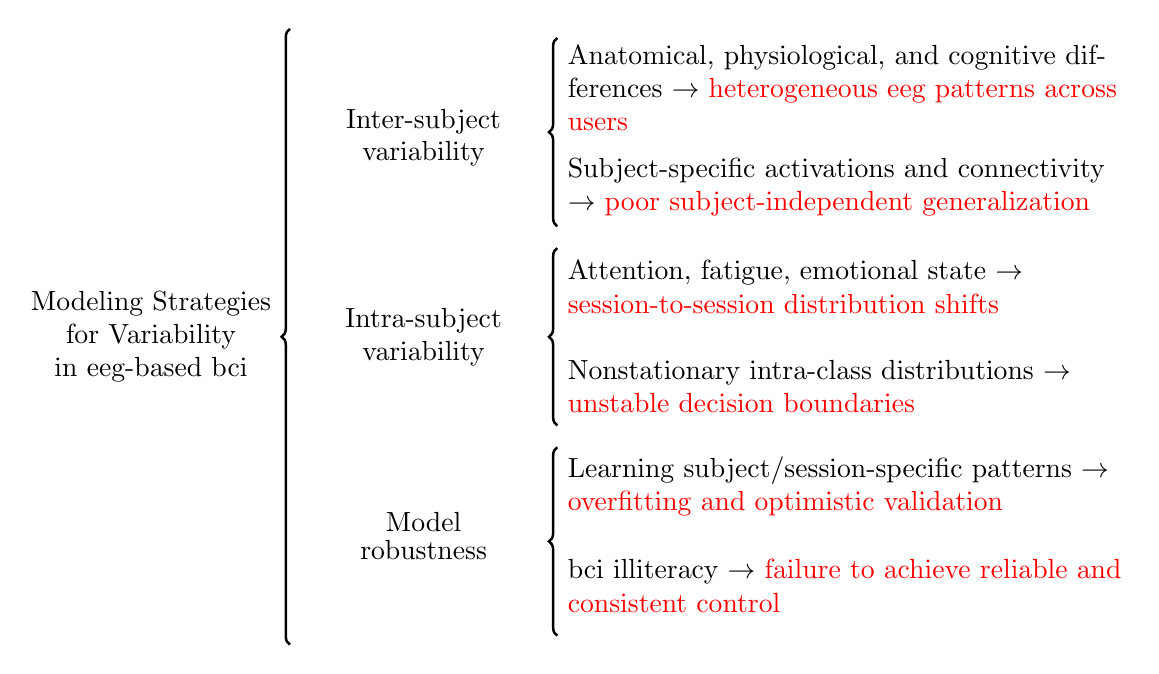
\begin{tikzpicture}[x=\linewidth,y=1.15cm,line width=0.9pt,font=\normalsize]

% ===== spacing =====
\def\labelpad{0.015}
\def\topbotMain{0.10}
\def\topbotInner{0.00}
\def\dy{1.1}
\def\yT{2.35}
\def\amp{3pt}
\def\vgap{0.12}

% ===== styles =====
\tikzset{
  brace/.style={
    draw=none,
    postaction={draw,decorate,decoration={brace,mirror,raise=0pt,amplitude=\amp}}
  },
  lab/.style={anchor=east,fill=white,inner sep=1.2pt,align=center},
  glab/.style={anchor=center,fill=white,inner sep=1.2pt,align=center},
  item/.style={anchor=west,text width=0.58\linewidth}
}

% ===== column positions =====
\pgfmathsetmacro{\xMain}{0.28}
\pgfmathsetmacro{\xInner}{0.56}
\pgfmathsetmacro{\xText}{0.56}
\pgfmathsetmacro{\xMid}{(\xMain+\xInner)/2}

% ===== main label =====
\def\Main{\shortstack{Modeling Strategies\\for Variability\\in \gls{eeg}-based \gls{bci}}}

% ===== group labels =====
\def\GOne{\shortstack{Inter-subject\\variability}}
\def\GTwo{\shortstack{Intra-subject\\variability}}
\def\GThree{\shortstack{Model\\robustness}}

% ===== items =====
\def\Ione{Anatomical, physiological, and cognitive differences $\rightarrow$ 
\textcolor{red}{heterogeneous \gls{eeg} patterns across users}}

\def\Itwo{Subject-specific activations and connectivity $\rightarrow$ 
\textcolor{red}{poor subject-independent generalization}}

\def\Ithree{Attention, fatigue, emotional state $\rightarrow$ 
\textcolor{red}{session-to-session distribution shifts}}

\def\Ifour{Nonstationary intra-class distributions $\rightarrow$ 
\textcolor{red}{unstable decision boundaries}}

\def\Ifive{Learning subject/session-specific patterns $\rightarrow$ 
\textcolor{red}{overfitting and optimistic validation}}

\def\Isix{\gls{bci} illiteracy $\rightarrow$ 
\textcolor{red}{failure to achieve reliable and consistent control}}

% ===== y positions =====
\pgfmathsetmacro{\yZero}{\yT}
\pgfmathsetmacro{\yOne}{\yT-1*\dy}
\pgfmathsetmacro{\yTwo}{\yT-2*\dy}
\pgfmathsetmacro{\yThree}{\yT-3*\dy}
\pgfmathsetmacro{\yFour}{\yT-4*\dy}
\pgfmathsetmacro{\yFive}{\yT-5*\dy}

% ===== main brace =====
\draw[brace] (\xMain,\yZero+0.5*\dy+\topbotMain) -- (\xMain,\yFive-0.5*\dy-\topbotMain);
\node[lab] at (\xMain-\labelpad,{(\yZero+\yFive)/2}) {\Main};

% ===== group braces =====
\draw[brace] (\xInner,\yZero+0.5*\dy+\topbotInner) --
             (\xInner,\yOne-0.5*\dy-\topbotInner+\vgap);

\draw[brace] (\xInner,\yTwo+0.5*\dy+\topbotInner-\vgap) --
             (\xInner,\yThree-0.5*\dy-\topbotInner+\vgap);

\draw[brace] (\xInner,\yFour+0.5*\dy+\topbotInner-\vgap) --
             (\xInner,\yFive-0.5*\dy-\topbotInner);

% ===== group labels =====
\node[glab] at (\xMid,{(\yZero+\yOne)/2}) {\GOne};
\node[glab] at (\xMid,{(\yTwo+\yThree)/2}) {\GTwo};
\node[glab] at (\xMid,{(\yFour+\yFive)/2}) {\GThree};

% ===== items =====
\node[item] at (\xText,\yZero) {\Ione};
\node[item] at (\xText,\yOne) {\Itwo};

\node[item] at (\xText,\yTwo) {\Ithree};
\node[item] at (\xText,\yThree) {\Ifour};

\node[item] at (\xText,\yFour) {\Ifive};
\node[item] at (\xText,\yFive) {\Isix};

\end{tikzpicture}
\vspace{-1.2em}
\caption{Summary of key factors motivating modeling strategies for handling inter- and intra-subject variability in \gls{eeg}-based \gls{bci} systems. Differences across users and sessions induce domain shift and overfitting, highlighting the need for robust subject-independent decoding frameworks.}
\label{fig:inter_intra_variability}
\end{figure}

A variety of modeling strategies have been proposed to address the pronounced inter- and intra-subject variability that limits the reliable deployment of \gls{eeg}-based \gls{bci} systems \cite{lotte2018review}. Inter-subject variability arises from anatomical, physiological, and neurocognitive differences between individuals \cite{kim2023bridging}, leading to heterogeneous \gls{eeg} patterns even when identical experimental paradigms are employed \cite{maswanganyi2022statistical}. In paradigms such as \gls{mi} and in \gls{eeg}-based applications targeting neurodevelopmental conditions, including \gls{adhd}, these differences manifest as subject-specific activation patterns, spectral characteristics, and connectivity structures, which substantially hinder the development of models capable of generalizing beyond the training population. {This variability, together with session-dependent shifts and robustness-related challenges, is summarized in Figure~\ref{fig:inter_intra_variability}.}

This variability poses a critical challenge for data-driven learning systems, as models trained on limited or homogeneous cohorts often exhibit significant performance degradation when evaluated on unseen subjects \cite{saha2020intra}. Such behavior indicates that many approaches inadvertently learn subject-specific or dataset-dependent artifacts rather than invariant neurophysiological structures \cite{lotte2018review}. Consequently, subject-independent decoding remains a largely unsolved problem, particularly in clinical and assistive \gls{bci} applications—including \gls{mi}-based systems and \gls{eeg}-based studies involving \gls{adhd}—where repeated calibration sessions are impractical or undesirable.

Several strategies have been proposed to mitigate variability-related challenges, including subject-specific calibration, transfer learning, and domain adaptation techniques \cite{al2025emotion}. While these methods can improve performance under constrained settings, they often rely on additional labeled data or assume a degree of similarity between source and target subjects that may not hold in practice. Moreover, many approaches focus primarily on classification accuracy, without explicitly addressing the stability and structure of the learned representations under distributional shifts \cite{wang2024dmmr}.

More recently, there has been growing interest in leveraging higher-level representations, such as functional and effective connectivity patterns, as potential carriers of invariant neurophysiological information \cite{faes2017information}. By modeling interactions between brain regions rather than isolated channel activity, connectivity-based representations may capture more stable organizational principles of brain function that are less sensitive to subject-specific variability. Nonetheless, existing implementations often remain decoupled from the learning process or lack mechanisms to enforce robustness and regularization at the representation level \cite{rolls2022effective}.

Taken together, these limitations highlight that current approaches to handling inter- and intra-subject variability remain insufficient to achieve robust subject-independent decoding in \gls{eeg}-based \gls{bci} systems \cite{lotte2018review,saha2020intra}. In particular, the lack of integrated frameworks that jointly address variability, representation stability, and generalization under distributional shifts continues to constrain real-world and clinical applicability. This gap motivates the development of learning paradigms capable of extracting stable and transferable representations that preserve discriminative information while remaining robust to subject- and session-dependent variations.

\subsection{Interpretability in \gls{eeg}-based Deep Learning}

In recent years, interpretability has emerged as a critical requirement in \gls{eeg}-based deep learning systems, particularly in applications related to neuroscience, clinical diagnosis, and neurorehabilitation~\cite{shoka2019literature}. While deep learning models have demonstrated superior performance compared to classical approaches, their black-box nature raises concerns regarding transparency, trustworthiness, and the physiological validity of the learned representations~\cite{bouazizi2024interpretability}. In the context of \gls{eeg}-based \glspl{bci}, interpretability is not merely a desirable property but a fundamental necessity, as decisions must be grounded in meaningful neural mechanisms rather than spurious correlations or artifacts.

Most existing efforts toward interpretability in \gls{eeg}-based deep learning rely on post-hoc explanation techniques, which aim to infer the relevance of input features after model training. Gradient-based attribution methods, such as Grad-CAM and its variants, have been widely adopted to highlight salient temporal segments or channels contributing to a given prediction \cite{samek2019explainable}. While these techniques provide intuitive visual explanations, they do not guarantee that the underlying representations correspond to genuine neurophysiological processes. Moreover, post-hoc explanations may be unstable under small perturbations of the input or model parameters, raising concerns about their reliability in high-variability \gls{eeg} scenarios \cite{bouazizi2024interpretability}. {The main interpretability limitations of current \gls{eeg}-based deep learning approaches are summarized in Figure~\ref{fig:interpretability_eeg_dl}.}

The limitations of post-hoc interpretability are particularly pronounced in \gls{eeg} analysis, where meaningful interpretation requires coherence across multiple dimensions, including spatial, temporal, and spectral domains. Explanations that focus solely on sensor-level activations may overlook the distributed and dynamic nature of brain activity, while failing to disentangle task-related neural patterns from noise or artifacts. As a result, post-hoc methods often provide only partial insight into model behavior, limiting their utility for validating neural plausibility or guiding clinical decision-making \cite{wang2019eeg}.

\begin{figure}[H]
\centering
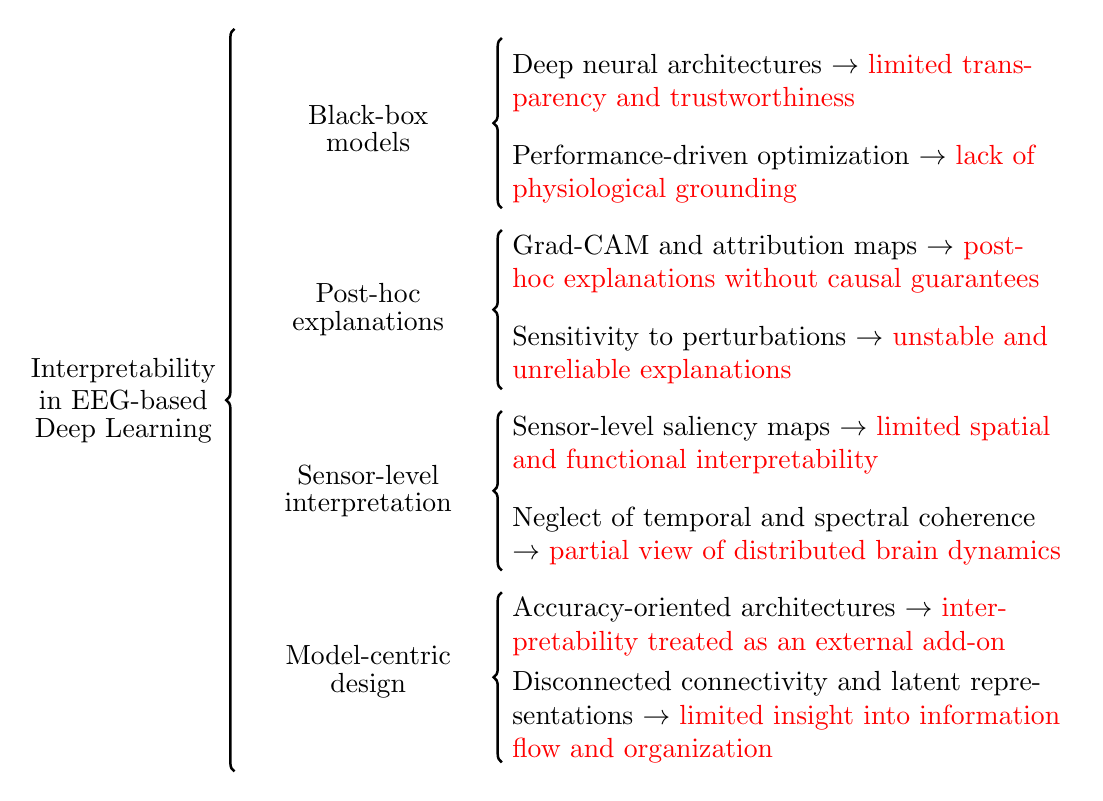
\begin{tikzpicture}[x=\linewidth,y=1.15cm,line width=0.9pt,font=\normalsize]

% ===== spacing =====
\def\labelpad{0.015}
\def\topbotMain{0.10}
\def\topbotInner{0.00}
\def\dy{1.0}
\def\yT{2.2}
\def\amp{3pt}
\def\vgap{0.12}

% ===== styles =====
\tikzset{
  brace/.style={
    draw=none,
    postaction={draw,decorate,decoration={brace,mirror,raise=0pt,amplitude=\amp}}
  },
  lab/.style={anchor=east,fill=white,inner sep=1.2pt,align=center},
  glab/.style={anchor=center,fill=white,inner sep=1.2pt,align=center},
  item/.style={anchor=west,text width=0.58\linewidth}
}

% ===== column positions =====
\pgfmathsetmacro{\xMain}{0.28}
\pgfmathsetmacro{\xInner}{0.56}
\pgfmathsetmacro{\xText}{0.56}
\pgfmathsetmacro{\xMid}{(\xMain+\xInner)/2}

% ===== main label =====
\def\Main{\shortstack{Interpretability\\in EEG-based\\Deep Learning}}

% ===== group labels =====
\def\GOne{\shortstack{Black-box\\models}}
\def\GTwo{\shortstack{Post-hoc\\explanations}}
\def\GThree{\shortstack{Sensor-level\\interpretation}}
\def\GFour{\shortstack{Model-centric\\design}}

% ===== items =====
\def\Ione{Deep neural architectures $\rightarrow$ 
\textcolor{red}{limited transparency and trustworthiness}}

\def\Itwo{Performance-driven optimization $\rightarrow$ 
\textcolor{red}{lack of physiological grounding}}

\def\Ithree{Grad-CAM and attribution maps $\rightarrow$ 
\textcolor{red}{post-hoc explanations without causal guarantees}}

\def\Ifour{Sensitivity to perturbations $\rightarrow$ 
\textcolor{red}{unstable and unreliable explanations}}

\def\Ifive{Sensor-level saliency maps $\rightarrow$ 
\textcolor{red}{limited spatial and functional interpretability}}

\def\Isix{Neglect of temporal and spectral coherence $\rightarrow$ 
\textcolor{red}{partial view of distributed brain dynamics}}

\def\Iseven{Accuracy-oriented architectures $\rightarrow$ 
\textcolor{red}{interpretability treated as an external add-on}}

\def\Ieight{Disconnected connectivity and latent representations $\rightarrow$ 
\textcolor{red}{limited insight into information flow and organization}}

% ===== y positions =====
\pgfmathsetmacro{\yZero}{\yT}
\pgfmathsetmacro{\yOne}{\yT-1*\dy}
\pgfmathsetmacro{\yTwo}{\yT-2*\dy}
\pgfmathsetmacro{\yThree}{\yT-3*\dy}
\pgfmathsetmacro{\yFour}{\yT-4*\dy}
\pgfmathsetmacro{\yFive}{\yT-5*\dy}
\pgfmathsetmacro{\ySix}{\yT-6*\dy}
\pgfmathsetmacro{\ySeven}{\yT-7*\dy}

% ===== main brace =====
\draw[brace] (\xMain,\yZero+0.5*\dy+\topbotMain) -- (\xMain,\ySeven-0.5*\dy-\topbotMain);
\node[lab] at (\xMain-\labelpad,{(\yZero+\ySeven)/2}) {\Main};

% ===== group braces =====
\draw[brace] (\xInner,\yZero+0.5*\dy+\topbotInner) --
             (\xInner,\yOne-0.5*\dy-\topbotInner+\vgap);

\draw[brace] (\xInner,\yTwo+0.5*\dy+\topbotInner-\vgap) --
             (\xInner,\yThree-0.5*\dy-\topbotInner+\vgap);

\draw[brace] (\xInner,\yFour+0.5*\dy+\topbotInner-\vgap) --
             (\xInner,\yFive-0.5*\dy-\topbotInner+\vgap);

\draw[brace] (\xInner,\ySix+0.5*\dy+\topbotInner-\vgap) --
             (\xInner,\ySeven-0.5*\dy-\topbotInner);

% ===== group labels =====
\node[glab] at (\xMid,{(\yZero+\yOne)/2}) {\GOne};
\node[glab] at (\xMid,{(\yTwo+\yThree)/2}) {\GTwo};
\node[glab] at (\xMid,{(\yFour+\yFive)/2}) {\GThree};
\node[glab] at (\xMid,{(\ySix+\ySeven)/2}) {\GFour};

% ===== items =====
\node[item] at (\xText,\yZero) {\Ione};
\node[item] at (\xText,\yOne) {\Itwo};

\node[item] at (\xText,\yTwo) {\Ithree};
\node[item] at (\xText,\yThree) {\Ifour};

\node[item] at (\xText,\yFour) {\Ifive};
\node[item] at (\xText,\yFive) {\Isix};

\node[item] at (\xText,\ySix) {\Iseven};
\node[item] at (\xText,\ySeven) {\Ieight};

\end{tikzpicture}
\vspace{-1.2em}
\caption{Key limitations of interpretability in \gls{eeg}-based deep learning. Existing approaches predominantly rely on black-box architectures and post-hoc explanations, which provide limited neurophysiological grounding, stability, and multi-dimensional coherence, constraining transparency and clinical reliability.}
\label{fig:interpretability_eeg_dl}
\end{figure}

In response to these challenges, recent research has emphasized the importance of interpretability by design, where model architectures are explicitly structured to reflect neurophysiological principles. Connectivity-based representations, latent space regularization, and reconstruction-driven learning have been proposed as mechanisms to embed interpretability directly into the learning process \cite{rolls2022effective}. By modeling interactions between brain regions or enforcing structured latent representations, these approaches facilitate the analysis of learned features in terms of functional organization and information flow, offering a more principled pathway toward explainable \gls{eeg} decoding \cite{faes2017information}.

Despite these advances, a significant gap remains in the development of integrated frameworks that jointly achieve high decoding performance, robustness to variability, and intrinsic interpretability. Many existing models prioritize accuracy while treating interpretability as a secondary or external concern, resulting in limited insight into the neural basis of model decisions \cite{lotte2018review}. This gap is particularly critical in scenarios characterized by high inter- and intra-subject variability, where interpretability plays a key role in identifying failure modes, understanding model generalization, and mitigating \gls{bci} illiteracy \cite{horowitz2021external}.

{In this context, \gls{bci} illiteracy, also referred to as \gls{bci} inefficiency, describes the difficulty experienced by a subset of users in producing sufficiently stable and discriminable neural patterns for reliable \gls{bci} control, despite training or repeated exposure. Several cognitive and user-centered hypotheses suggest that this phenomenon may be related to inter-individual differences in attention, fatigue, motivation, mental workload, motor-imagery vividness, spatial abilities, and the capacity to consistently modulate sensorimotor rhythms~\cite{jeunet2015predicting,leeuwis2021vividness,ahn2013high}. From this perspective, interpretable models may help identify whether poor \gls{bci} performance arises from weak task-related neural modulation, unstable connectivity patterns, or model-specific failure modes.}

Overall, the lack of robust and neurophysiologically grounded interpretability remains a major limitation of current \gls{eeg}-based deep learning approaches \cite{bouazizi2024interpretability}. Addressing this issue requires models that not only perform accurate classification but also provide transparent and multi-dimensional explanations of their internal representations. Such frameworks are essential for ensuring the reliability, clinical relevance, and ethical deployment of \gls{eeg}-based \gls{bci} systems, motivating the development of methods that integrate interpretability as a core design principle rather than an afterthought.

\subsection{Summary}

{The state-of-the-art analysis shows that \gls{eeg}-based \gls{bci} research has evolved from classical signal-processing pipelines toward deep learning and connectivity-driven approaches. Although handcrafted features, deep neural architectures, and connectivity measures have each contributed to improving \gls{mi} decoding, they still face important limitations related to the low spatial resolution of \gls{eeg}, noise sensitivity, nonlinear and nonstationary brain dynamics, and limited generalization across subjects and sessions.}

{A central challenge identified across the literature is the lack of integrated frameworks capable of jointly addressing inter- and intra-subject variability, connectivity modeling, robustness, and interpretability. Existing methods often optimize these aspects separately: classical approaches depend on manual feature extraction, many deep learning models remain mainly sensor-driven and vulnerable to overfitting, and connectivity-based methods are frequently decoupled from end-to-end representation learning.}

{In addition, variability in neural patterns contributes to the \gls{bci} illiteracy phenomenon, in which a subset of users fails to achieve reliable \gls{bci} control despite training or repeated exposure. This limitation may be associated not only with neurophysiological variability, but also with cognitive and user-related factors such as attention, fatigue, motivation, mental workload, clarity or vividness of motor imagery, and the ability to consistently modulate sensorimotor rhythms.}

{Overall, the reviewed literature highlights the need for learning approaches that jointly model nonlinear and time-varying brain connectivity, improve robustness and generalization, and provide interpretable representations grounded in neurophysiological principles. Addressing these challenges constitutes the main motivation for the proposed doctoral research.}


